\part{Constitutive Theory}
\label{partConstitutive}

Roan \& Waters \cite{RoanWaters11} and Suki \textit{et~al}.\ \cite{Sukietal05,Sukietal11} have each written extensive review articles on the mechanics of parenchyma, have provided detailed information about the structural constituents of alveoli, and have discussed their influence on the overall mechanical response of parenchyma.  Of particular relevance, from a mechanics perspective, are the constituent building blocks of alveolar tissue: collagen (types I and III, predominantly), elastin, proteoglycans and other proteins, surfactant and cells (epithelial and endothelial, predominantly).  These constituents are assembled in such a manner so as to produce a variety of alveolar sub-structures that are essentially 1D (alveolar chords), 2D (alveolar septa) and 3D (alveolar sacs) in their geometric construction.

A dodecahedron is used here as a geometric model for an alveolus \cite{FrankusLee74}, cf.\ Figs.~\ref{figRatLung} \& \ref{figDodecahedron}.  It is comprised of: thirty 1D rods that represent alvolar chords, twelve 2D membranes that represent alveolar septa, considered here to be pentagonal in shape, and one 3D cavity filled with air (or fluids in the case of a contusion caused by injury or an edema caused by disease), considered here to be dodecahedral in shape.  The thermo\-elastic constitutive equations presented in this chapter for these three spatial geometries are derived in \ref{appImplicitElasticity}.  Elastic behavior is sufficient for our intended application of studying alveoli being subjected to traveling waves.

We recall from our kinematic study of a dodecahedron that the geometric strains of $e \defeq \ln ( L / L_0 )$ for the elongation of septal chords, $\xi \defeq \ln \sqrt{A / A_0}$ for the dilation of septal membranes, and $\Xi \defeq \ln \sqrt[3]{V / V_0}$ for the dilatation of alveolar volume are equivalent to one another under motions of uniform expansion.  These three, geometric, strain measures also exist as thermo\-dynamic strains, each associating with a distinct and unique conjugate stress.

Constitutive equations are a derived consequence from physical laws governing thermo\-dynamic processes.  Here we derive constitutive equations applicable for 1D thermo\-elastic fibers (alveolar chords), 2D thermo\-elastic membranes (alveolar septa), and 3D thermo\-elastic volumes (alveolar sacs).  In \S\ref{secUniformCE}, we assume that the motions are uniform in their spatial dimension.  Later, in \S\ref{secNonuniform2D}, the non-uniform motions of shears associated with a membrane are included into this thermo\-dynamic framework.  Section~\ref{secAlveolus} pulls these results together, sufficient for the intended purpose of modeling the three structural facets that comprise an alveolous.  Specifically, all geometric entities (alveolar chords, alveolar septa, and alveolar sacs) are described in terms of stresses ($\text{dyne/cm}^2$) instead of their intensive thermo\-dynamic forces (force, surface tension, and stress).  This is done to facilitate implementation of these models into code, and to facilitate interpretations of their results by engineers and scientists.

\section{Green Thermoelastic Solids Subjected to Uniform Motions in 1D, 2D \& 3D}
\label{secUniformCE}

Combining the First and Second Laws of Thermo\-dynamics governing uniform, reversible, adiabatic processes results in the following three formul\ae, one per dimension; they are
\begin{subequations}
    \label{thermoelasticLaws}
    \begin{align}
    \mbox{} & \text{In 1 Dimension:} & 
    \mathrm{d}U & = \theta \, \mathrm{d} \eta +
    \tfrac{1}{\rho_{1D}} F \, \mathrm{d}L / L
    \label{thermoelastic1Dlaw} \\
    \mbox{} & \text{In 2 Dimensions:} &
    \mathrm{d}U & = \theta \, \mathrm{d} \eta + 
    \tfrac{1}{\rho_{2D}} T \, \mathrm{d}A / \! A
    \label{thermoelastic2Dlaw} \\
    \mbox{} & \text{In 3 Dimensions:} &
    \mathrm{d}U & = \theta \, \mathrm{d} \eta - 
    \tfrac{1}{\rho_{3D}} P \, \mathrm{d}V \! / V \!
    \label{thermoelastic3Dlaw}
    \end{align}
\end{subequations}
wherein $U$ is an internal energy density (erg/gr = dyne.cm/gr), which is a function of state, $\theta$ is a temperature in Kelvin ($273 + \mbox{}^{\circ}$C), $\eta$ is an entropy density (erg/gr.K), $L$ is a length of line (cm), $A$ is an area of surface ($\text{cm}^2$), $V$ is a volume in space ($\text{cm}^3$), $F$ is a force (dyne), $T$ is a surface tension (dyne/cm), and $P$ is a pressure (dyne/$\text{cm}^2$ = barye), whereas the mass densities $\rho_{1D}$ ($\text{gr/cm}$), $\rho_{2D}$ ($\text{gr/cm}^2$) and $\rho_{3D}$ ($\text{gr/cm}^3$) associate with a reference state of per unit length, or per unit area, or per unit volume, as appropriate.  Pressure $P$ is assigned to be positive whenever a body undergoes hydro\-static compression, per accepted practice.

\subsection{Constitutive Equations}

Because the internal energy density $U$ is a state function, its total derivative describes a Pfaffian form \cite{Caratheodory09} out of which the following constitutive formul\ae\ are readily obtained
\begin{subequations}
    \label{GreenElasticCEs}
    \begin{align}
    \mbox{} & \text{In 1 Dimension:} & 
    \theta & = \partial_{\eta} U ( \eta , e) &
    F & = \rho_{1D} \, \partial_{e} U ( \eta , e) \\
    \mbox{} & \text{In 2 Dimensions:} &
    \theta & = \partial_{\eta} U ( \eta , \xi) &
    2T & = \rho_{2D} \, \partial_{\xi} U ( \eta , \xi) \\
    \mbox{} & \text{In 3 Dimensions:} &
    \theta & = \partial_{\eta} U ( \eta ,  \Xi) &
    -3P & = \rho_{3D} \, \partial_{\Xi} U ( \eta ,  \Xi)
    \end{align}
\end{subequations}
where we have used the geometric strain definitions $e \defeq \ln ( L / L_0 )$, $\xi \defeq \ln \sqrt{ A / \! A_0 }$ and $\Xi \defeq \sqrt[3]{V \! / V_0}$, in accordance with Part~\ref{partKinematics}. These constitutive equations govern Green thermo\-elastic solids undergoing uniform motions in adiabatic enclosures.  As a convenience, we employ the following notation $\partial_{\eta} U \defeq \partial U / \partial \eta$, etc.

Consider the response variables for temperature and force\slash surface-tension\slash pressure to be $C^1$ functions of state (cf.\ Weinhold \cite{Weinhold75c} and Gilmore \cite{Gilmore84}) in a Green thermo\-elastic solid undergoing an uniform adiabatic motion.  One can then differentiate Eqn.~(\ref{GreenElasticCEs}), thereby producing the following collection of coupled differential equations
\begin{subequations}
    \label{GreenElasticODEs}
    \begin{align}
    \mbox{} & \text{In 1 Dimension:} &
    \left\{ \begin{matrix} \mathrm{d} \theta \\ 
    \mathrm{d} F \end{matrix} \right\} & = \begin{bmatrix}
    \partial_{\eta\eta} U & \partial_{\eta e} U \\
    \rho_{1D} \, \partial_{e\eta} U & \rho_{1D} \, \partial_{ee} U \end{bmatrix} 
    \left\{ \begin{matrix} \mathrm{d} \eta \\
    \mathrm{d} e \end{matrix} \right\} \\
    % second formula
    \mbox{} & \text{In 2 Dimensions:} &
    \left\{ \begin{matrix} \mathrm{d} \theta \\ 
    2 \, \mathrm{d} T \end{matrix} \right\} & = \begin{bmatrix}
    \partial_{\eta\eta} U & \partial_{\eta \xi} U \\
    \rho_{2D} \, \partial_{\xi\eta} U & \rho_{2D} \, \partial_{\xi\xi} U \end{bmatrix} \left\{ \begin{matrix} \mathrm{d} \eta \\
    \mathrm{d} \xi \end{matrix} \right\} \label{GreenMembrane} \\
    % third formula
    \mbox{} & \text{In 3 Dimensions:} &
    \left\{ \begin{matrix} \mathrm{d} \theta \\ 
    -3 \, \mathrm{d} P \end{matrix} \right\} & = \begin{bmatrix}
    \partial_{\eta\eta} U & \partial_{\eta \Xi} U \\
    \rho_{3D} \, \partial_{\Xi\eta} U & \rho_{3D} \, \partial_{\Xi\Xi} U \end{bmatrix} \left\{ \begin{matrix} \mathrm{d} \eta \\
    \mathrm{d} \Xi \end{matrix} \right\}
    \end{align}
\end{subequations}
where, from calculus, mixed partial derivatives obey $\partial_{e\eta} U = \partial^2 U / \partial e \partial \eta = \partial^2 U / \partial \eta \partial e = \partial_{\eta e} U$, etc., that in the thermo\-dynamics literature are known as Maxwell's relations; they are Silvester's criteria for integrability.

Changing cause and effect between entropy and temperature in Eqn.~(\ref{GreenElasticODEs}) leads to
\begin{subequations}
    \label{HelmholtzElasticODEs}
    \begin{align}
    \left\{ \begin{matrix} \mathrm{d} \eta \\ 
    \mathrm{d} F \end{matrix} \right\} & = \begin{bmatrix}
    1/\partial_{\eta\eta} U & -\partial_{\eta e} U / 
    \partial_{\eta\eta} U \\
    \rho_{1D} \, \partial_{e\eta} U / \partial_{\eta\eta} U & \rho_{1D} ( \partial_{ee} U - \partial_{e\eta} U \!\cdot\! \partial_{\eta e} U / \partial_{\eta\eta} U ) \end{bmatrix} 
    \left\{ \begin{matrix} \mathrm{d} \theta \\
    \mathrm{d} e \end{matrix} \right\} \\
    % second formula
    \left\{ \begin{matrix} \mathrm{d} \eta \\ 
    2 \, \mathrm{d} T \end{matrix} \right\} & = \begin{bmatrix}
    1/\partial_{\eta\eta} U & -\partial_{\eta \xi} U / \partial_{\eta\eta} U \\
    \rho_{2D} \, \partial_{\xi\eta} U / \partial_{\eta\eta} U & \rho_{2D} ( \partial_{\xi\xi} U - \partial_{\xi\eta} U \!\cdot\! \partial_{\eta\xi} U / \partial_{\eta\eta} U ) \end{bmatrix} \left\{ \begin{matrix} \mathrm{d} \theta \\
    \mathrm{d} \xi \end{matrix} \right\} \label{HelmholtzMembrane} \\
    % thrid formula
    \left\{ \begin{matrix} \mathrm{d} \eta \\ 
    -3 \, \mathrm{d} P \end{matrix} \right\} & = \begin{bmatrix}
    1/\partial_{\eta\eta} U & -\partial_{\eta \Xi} U / \partial_{\eta\eta} U \\
    \rho_{3D} \, \partial_{\Xi\eta} U / \partial_{\eta\eta} U & \rho_{3D} ( \partial_{\Xi\Xi} U - \partial_{\Xi\eta} U \!\cdot\! \partial_{\eta\Xi} U / \partial_{\eta\eta} U ) \end{bmatrix} \left\{ \begin{matrix} \mathrm{d} \theta \\
    \mathrm{d} \Xi \end{matrix} \right\}
    \end{align}
\end{subequations}
which are written above in a format that is more useful for our multi\-scale application.  In this process, a localization procedure pulls temperature and strain from the continuum scale down to the alveolar scale.  The alveolar entropy and stress are then determined via the above constitutive equations.  Afterwords, an homogenization procedure pushes the updated alveolar entropy and stress up to the continuum level.  We employ the independent variables of a Helmholtz free energy, but we do not adopt his potential, preferring to retain the internal energy potential to ensure a proper incorporation of Maxwell's constraint.  

Constitutive equations (\ref{GreenElasticODEs} \& \ref{HelmholtzElasticODEs}) take on the form of hypo-elastic material models \cite{Truesdell55}, which are ideal for numerical implementation whenever one uses numerical solution techniques like those presented in Part~\ref{partNumericalMethods}.

\subsection{Material Constants}

Experiments are performed for the purpose of characterizing material behavior.  In mechanics, we relate measured material constants to gradients and curvatures of thermo\-dynamic potentials out of which material models are created.  Experiments are typically done to quantify the following material constants, selected per a material's physical dimension:
\begin{subequations}
\label{materialConstants}
\begin{align}
C_f & \defeq \theta \, \partial_{\theta} \eta |_F & 
\alpha_f & \defeq L^{-1} \, \partial_{\theta} L |_F = 
\partial_{\theta} e |_F &
E_{\theta} & \defeq L \, \partial_L F |_{\theta} = 
\partial_e F |_{\theta} \\
C_t & \defeq \theta \, \partial_{\theta} \eta |_T & 
\alpha_t & \defeq A^{-1} \, \partial_{\theta} A |_T = 
2 \, \partial_{\theta} \xi |_T &
M_{\theta} & \defeq A \, \partial_A T |_{\theta} = 
\tfrac{1}{2} \, \partial_{\xi} T |_{\theta} \\
C_p & \defeq \theta \, \partial_{\theta} \eta |_P & 
\alpha_p & \defeq V^{-1} \, \partial_{\theta} V |_P = 
3 \, \partial_{\theta} \Xi |_P &
-K_{\theta} & \defeq V \, \partial_V P |_{\theta} = 
\tfrac{1}{3} \, \partial_{\Xi} P |_{\theta}
\end{align}
\end{subequations}
Herein, the various specific heats $C_f$, $C_t$, $C_p$ (erg/gr.K) are, essentially,  all equivalent as they are all defined per unit mass, insensitive to dimension.  Hereafter they will be denoted simply as $C$.  However, the various thermal expansions $\alpha_f$, $\alpha_t$, $\alpha_p$ (1/K) are all distinct, as they are each defined with respect to their physical dimension, viz., $\alpha_f \defeq L^{-1} \, \partial L / \partial \theta |_F$, $\alpha_t \defeq A^{-1} \, \partial A / \partial \theta |_T$ and $\alpha_p \defeq V^{-1} \, \partial V / \partial \theta |_P$.  Parameter $E_{\theta}$ is a modulus of extension (dyne), parameter $M_{\theta}$ is a modulus of dilation (dyne/cm), and parameter $K_{\theta}$ is a modulus of dilatation ($\mathrm{dyne/cm}^2$), a.k.a.\ the bulk modulus, with each modulus being measured at fixed temperature.  Shear moduli are discussed later in \S\ref{secNonuniform2D}.  The above material constants are gradients; they constitute tangents to their associated physical response curves.  Consequently, they need not be of constant value throughout state space, like a Hookean material supposes them to be.  This is an important characteristic for our application.  Here we employ the commonly used notation $\partial_{\theta} \eta |_F \defeq ( \partial \eta / \partial \theta ) |_F$, etc.

In terms of the material constants given in Eqn.~(\ref{materialConstants}), of which there are three per dimension, the internal energy density has the following three curvatures associated with it.  For 1D materials:
\begin{subequations}
    \label{internalEnergies}
    \begin{align}
    % for 1D materials
    \partial_{\eta\eta} U & = 
    \frac{\rho_{1D}\theta}{\rho_{1D} C - E_{\theta} \alpha_f^2 \theta } \\
    \partial_{ee} U & = \frac{C E_{\theta}}
    {\rho_{1D} C - E_{\theta} \alpha_f^2 \theta} \\
    \partial_{\eta e} U \equiv \partial_{e \eta} U & = 
    \frac{-E_{\theta} \alpha_f \theta}{\rho_{1D} C - E_{\theta} \alpha_f^2 \theta} \\
    \intertext{For 2D materials:}
    \partial_{\eta\eta} U & = 
    \frac{\rho_{2D} \theta}{\rho_{2D} C - M_{\theta} \alpha_t^2 \theta} \\
    \partial_{\xi\xi} U & = \frac{4 C M_{\theta}}
    {\rho_{2D} C - M_{\theta} \alpha_t^2 \theta} \\
    \partial_{\eta \xi} U \equiv \partial_{\xi \eta} U & = 
    \frac{-2M_{\theta} \alpha_t \theta}
    {\rho_{2D} C - M_{\theta} \alpha_t^2 \theta} \\
    \intertext{For 3D materials (cf.\ Weinhold \cite{Weinhold75c} and Gilmore \cite{Gilmore84}):}
    \partial_{\eta\eta} U & = 
    \frac{\rho_{3D} \theta}{\rho_{3D} C - K_{\theta} \alpha_p^2 \theta} \\
    \partial_{\Xi\Xi} U & = \frac{9 C K_{\theta}}
    {\rho_{3D} C - K_{\theta} \alpha_p^2 \theta} \\
    \partial_{\eta\Xi} U \equiv 
    \partial_{\Xi\eta} U & = 
    \frac{-3K_{\theta} \alpha_p \theta}{\rho_{3D} C - K_{\theta} \alpha_p^2 \theta}
    \end{align}
\end{subequations}
These materials constants are constrained by thermo\-dynamics in that
\begin{equation}
    \label{thermodynamicConstraints}
    0 < E_{\theta} < \frac{\rho_{1D} C}{\alpha_f^2 \, \theta} \qquad
    0 < M_{\theta} < \frac{\rho_{2D} C}{\alpha_t^2 \, \theta} \qquad
    0 < K_{\theta} < \frac{\rho_{3D} C}{\alpha_p^2 \, \theta}
\end{equation} 
which ensure that their respective thermo\-dynamic Jacobians cannot become singular. Singularities can and do occur, e.g., during a phase change in a crystal \cite{McLellan76,Gilmore84}, but such processes are not expected to arise in our application.

\subsection{Thermoelastic Models Suitable for Modeling Alveoli Subjected to Uniform Motions}

We now write down our constitutive formul\ae\ for quantifying uniform responses in thermo\-elastic solids of 1, 2 or 3 dimensions.  They are the thermo\-elastic constitutive equations (\ref{HelmholtzElasticODEs}) with Helmholtz variables expressed in terms of the material constants defined in Eqn.~(\ref{materialConstants}) assigned to the internal energy density $U$ according to Eqn.~(\ref{internalEnergies}), with outcomes of
\begin{subequations}
    \label{HelmholtzCEs}
    \begin{align}\
    \text{For 1D Materials:} & &
    \left\{ \begin{matrix}
    \mathrm{d} \eta \\ \mathrm{d} F
    \end{matrix} \right\} & = \begin{bmatrix}
    C / \theta - E_{\theta} \alpha_f^2 / \rho_{1D}& 
    E_{\theta} \alpha_f / \rho_{1D} \\
    -E_{\theta} \alpha_f & E_{\theta}
    \end{bmatrix} \left\{ \begin{matrix}
    \mathrm{d} \theta \\ \mathrm{d} e
    \end{matrix} \right\} \label{Helmholtz1D} \\
    % the second equation
    \text{For 2D Materials:} & &
    \left\{ \begin{matrix}
    \mathrm{d} \eta \\ 2 \, \mathrm{d} T
    \end{matrix} \right\} & = \begin{bmatrix}
    C / \theta - M_{\theta} \alpha_t^2 / \rho_{2D} & 
    2 M_{\theta} \alpha_t / \rho_{2D} \\
    -2 M_{\theta} \alpha_t & 4 M_{\theta}
    \end{bmatrix} \left\{ \begin{matrix}
    \mathrm{d} \theta \\ \mathrm{d} \xi
    \end{matrix} \right\} \label{Helmholtz2D} \\
    % the third equation
    \text{For 3D Materials:} & &
    \left\{ \begin{matrix}
    \mathrm{d} \eta \\ -3 \, \mathrm{d} P
    \end{matrix} \right\} & = \begin{bmatrix}
    C / \theta - K_{\theta} \alpha_p^2 / \rho_{3D} & 
    3 K_{\theta} \alpha_p / \rho_{3D} \\
    -3K_{\theta} \alpha_p & 9 K_{\theta}
    \end{bmatrix} \left\{ \begin{matrix}
    \mathrm{d} \theta \\ \mathrm{d} \Xi
    \end{matrix} \right\} \label{Helmholtz3D}
    \end{align}
\end{subequations}
These constitutive formul\ae, derived from the First and Second Laws of Thermo\-dynamics, describe thermo\-elastic materials undergoing uniform motions through adibatic processes.

The whole upper-left component in each matrix of Eqn.~(\ref{HelmholtzCEs}) represents a specific heat evaluated at constant strain, divided by temperature---a material property not easily measured.  Whereas, the specific heat evaluated at constant pressure, viz., $C$, is more amenable to experiments, and is the property that one typically finds in published data tables.  

There are four material constants for each dimension (e.g., for 1D materials they are: $\rho_{1D}$, $C$, $\alpha_f$ and $E_{\theta}$) with the latter three being defined according to Eqn.~(\ref{materialConstants}).  The differential equations in Eqn.~(\ref{HelmholtzCEs}) have mathematical forms of hypo-elastic materials \cite{Truesdell55}, which are preferred for incorporating constitutive equations into finite element packages.

\section{Green Thermoelastic Membranes Subjected to Non-Uniform Motions}
\label{secNonuniform2D}

For modeling healthy alveolar geometry via a dodecahedron, only the septal membranes are considered as  being capable of supporting shears, and therefore, only they need to have their constitutive structure extended to include the non-uniform motions of shear, of which pure shears (squeeze) are likely to dominate over simple shears.

The First and Second Laws of Thermo\-dynamics governing a reversible adiabatic process are described by the formula $\mathrm{d}\hspace{1pt}U = \theta \, \mathrm{d} \eta + \tfrac{1}{\rho} \, \mathrm{d}W$, where $\mathrm{d}W$ is the mechanical power expended by stressing a body of mass density $\rho$.  For the case of a 2D planar membrane, a mass density of $\rho \Leftarrow \rho_{2D}$ applies, with its change in mechanical work being expressed as \cite{Freedetal17,FreedZamani19,Freedetal20}
\begin{subequations}
\begin{align}
\mathrm{d} W & = \mathrm{tr} \left( 
\begin{bmatrix}
\mathcal{S}_{11} & \mathcal{S}_{12} \\
\mathcal{S}_{21} & \mathcal{S}_{22}
\end{bmatrix} \begin{bmatrix}
\mathrm{d}a / a & a \, \mathrm{d} g / b \\
0 & \mathrm{d}b / b 
\end{bmatrix} \right) =  
\pi \, \mathrm{d} \xi + \sigma \, \mathrm{d} \varepsilon + 
\tau \, \mathrm{d} \gamma
\label{convectedWorkRate} \\
\intertext{wherein the $\mathcal{S}_{ij}$ are components of a surface tension evaluated in the co-ordinate frame of a membrane.  (In \S\ref{secAlveolus} they will be converted into components of the second Piola-Kirchhoff stress.)  Therefore, the First and Second Laws result in an exact differential equation of the form}
\mathrm{d} \hspace{1pt} U & = \theta \, \mathrm{d} \eta + \tfrac{1}{\rho_{2D}} 
\bigl( \pi \, \mathrm{d} \xi + \sigma \, \mathrm{d} \varepsilon + 
\tau \, \mathrm{d} \gamma \bigr)
\label{membraneThermo}
\end{align}
\end{subequations} 
where $\{ \pi , \sigma , \tau  \}$ describes a set of intensive scalar-valued stresses whose thermo\-dynamic conjugates $\{ \xi , \varepsilon , \gamma \}$ describe a set of extensive scalar-valued strains.  (This contrasts with the classic approach where the work done is decomposed into a scalar-valued isotropic part and a tensor-valued deviatoric part.)  Pair $( \xi , \pi )$ describes a dilation $\xi$ caused by a surface tension $T$; it is the uniform contribution to stress power discussed in \S\ref{secUniformCE} where $2 \, \mathrm{d} \xi \Leftarrow A^{-1} \, \mathrm{d} A$ and $\tfrac{1}{2} \pi \Leftarrow T$.  Pair $( \varepsilon , \sigma )$ describes a pure shear $\varepsilon$ or squeeze caused by a normal-stress difference $\sigma$.  And pair $( \gamma , \tau )$ describes an in-plane shear $\gamma$ caused by a shear stress $\tau$. Collectively, pairs $( \varepsilon , \sigma )$ and $( \gamma , \tau )$ account for any non-uniform contributions to stress power, i.e., contributions from other than uniform dilation.  These pairs are quantified in \S\ref{secConjugatePairs}.

\subsection{Constitutive Equations}

Because a change in the internal energy $\mathrm{d} \hspace{1pt} U$ governing a reversible adiabatic process is described by an exact differential \cite{Caratheodory09}, with $U( \eta, \xi, \varepsilon, \gamma )$ in the case of a planar membrane, it follows that a constitutive response for a Green thermo\-elastic membrane is given by
\begin{subequations}
    \label{GreenThermoelasticity}
    \begin{align}
    \theta & = \partial_{\eta} U(\eta, \xi, \varepsilon, \gamma) , \;
    \phantom{\rho}
    \pi = \rho \, \partial_{\xi} U(\eta, \xi, \varepsilon, \gamma) ,
    \notag \\
    \sigma & = \rho \, \partial_{\varepsilon} U(\eta, \xi, \varepsilon, \gamma) , \;
    \tau = \rho \, \partial_{\gamma} U(\eta, \xi, \varepsilon, \gamma)
    \label{GreenThermoelasticMembrane} \\
    \intertext{with strain symmetries requiring that}
    U(\eta, \xi, \varepsilon, \gamma) & =
    U(\eta, \xi, -\varepsilon, \gamma) = 
    U(\eta, \xi, \varepsilon, -\gamma) = 
    U(\eta, \xi, -\varepsilon, -\gamma) .
    \label{internalEnergyInveriance}
    \end{align}
\end{subequations}
Considering that each intensive variable, viz., $\theta$, $\pi$, $\sigma$ and $\tau$, is actually a $C^1$ function of the set of extensive variables ($\eta , \xi , \varepsilon , \gamma$), then the constitutive expressions in Eqn.~(\ref{GreenThermoelasticMembrane}) can be recast into the following system of differential equations
\begin{equation}
\label{energies2D}
\left\{ \begin{matrix}
\mathrm{d} \theta \\ \mathrm{d} \pi \\
\mathrm{d} \sigma \\ \mathrm{d} \tau
\end{matrix} \right\} = \begin{bmatrix}
\partial_{\eta\eta} U & 
\partial_{\eta\xi} U & 
\partial_{\eta\varepsilon} U & 
\partial_{\eta\gamma} U \\ 
\rho \, \partial_{\xi\eta} U & 
\rho \, \partial_{\xi\xi} U & 
\rho \, \partial_{\xi\varepsilon} U &
\rho \, \partial_{\xi\gamma} U \\
\rho \, \partial_{\varepsilon\eta} U & 
\rho \, \partial_{\varepsilon\xi} U & 
\rho \, \partial_{\varepsilon\varepsilon} U & 
\rho \, \partial_{\varepsilon\gamma} U \\
\rho \, \partial_{\gamma\eta} U & 
\rho \, \partial_{\gamma\xi} U & 
\rho \, \partial_{\gamma\varepsilon} U & 
\rho \, \partial_{\gamma\gamma} U 
\end{bmatrix} 
\left\{ \begin{matrix}
\mathrm{d}\eta \\ \mathrm{d} \xi \\
\mathrm{d} \varepsilon \\ \mathrm{d} \gamma
\end{matrix} \right\}  
\end{equation}
whose upper-left $2\times 2$ sub-matrix also appears in Eqn.~(\ref{GreenMembrane}), which governs the uniform contribution of a response.  The above $4 \times 4$ matrix describes the full non-uniform response permissible by a Green thermo\-elastic membrane undergoing an adiabatic process.

For our application, it is reasonable to assume that the presence of a non-uniform planar motion will not cause an uniform planar response.  Said differently, it is reasonable to assume that pure $\varepsilon$ and simple $\gamma$ shears will not effect a change in either temperature $\theta$ or surface tension $\pi$.  Consequently, $\partial_{\eta\varepsilon} U = \partial_{\eta\gamma} U = \partial_{\xi\varepsilon} U = \partial_{\xi\gamma} U = 0$, and Eqn.~(\ref{energies2D}) simplifies to
\begin{displaymath}
\left\{ \begin{matrix}
\mathrm{d} \theta \\ \mathrm{d} \pi \\
\mathrm{d} \sigma \\ \mathrm{d} \tau
\end{matrix} \right\} = \begin{bmatrix}
\partial_{\eta\eta} U & 
\partial_{\eta\xi} U & 
0 & 0 \\ 
\rho \, \partial_{\xi\eta} U & 
\rho \, \partial_{\xi\xi} U & 
0 & 0 \\
0 & 0 & 
\rho \, \partial_{\varepsilon\varepsilon} U & 
\rho \, \partial_{\varepsilon\gamma} U \\
0 & 0 & 
\rho \, \partial_{\gamma\varepsilon} U & 
\rho \, \partial_{\gamma\gamma} U 
\end{bmatrix} 
\left\{ \begin{matrix}
\mathrm{d}\eta \\ \mathrm{d} \xi \\
\mathrm{d} \varepsilon \\ \mathrm{d} \gamma
\end{matrix} \right\} 
\end{displaymath}
with $\partial_{\varepsilon\eta} U = \partial_{\gamma\eta} U = \partial_{\varepsilon\xi} U = \partial_{\gamma\xi} U = 0$ because of Maxwell's relations.  Converting the above internal energy formulation into its Helmholtz equivalent results in
\begin{equation}
\left\{ \begin{matrix}
\mathrm{d} \eta \\ \mathrm{d} \pi \\
\mathrm{d} \sigma \\ \mathrm{d} \tau
\end{matrix} \right\} = \begin{bmatrix}
1 / \partial_{\eta\eta} U & 
-\partial_{\eta\xi} U / \partial_{\eta\eta} U & 
0 & 0 \\ 
\rho \, \partial_{\xi\eta} U / \partial_{\eta\eta} U & 
\rho \bigl( \partial_{\xi\xi} U - \partial_{\xi\eta} U \!\cdot\! \partial_{\eta\xi} U / \partial_{\eta\eta} U \bigr) & 0 & 0 \\
0 & 0 & \rho \, \partial_{\varepsilon\varepsilon} U & 
\rho \, \partial_{\varepsilon\gamma} U \\
0 & 0 & \rho \, \partial_{\gamma\varepsilon} U & 
\rho \, \partial_{\gamma\gamma} U 
\end{bmatrix} 
\left\{ \begin{matrix}
\mathrm{d}\theta \\ \mathrm{d} \xi \\
\mathrm{d} \varepsilon \\ \mathrm{d} \gamma
\end{matrix} \right\}  
\label{Helmholtz2Duncoupled}
\end{equation}
which provides the general structure for a Green thermo\-elastic membrane appropriate for our application.  The uniform response (the upper-left $2 \times 2$ sub-matrix) and the non-uniform response (the lower-right $2 \times 2$ sub-matrix) are, by conjecture, decoupled in this constitutive construction.

\medskip\noindent
\textbf{Note}: There is experimental evidence that the bulk and shear moduli of parenchyma both depend upon transpulmonary pressure \cite{LaiFook79,Jahedetal90}.  It is conjectured that this is a structural effect of alveolar geometry; it is not a characteristic of the constituents that comprise an alveolus.  As such, we do not couple the uniform and non-uniform responses in Eqn.~(\ref{Helmholtz2Duncoupled}).

\subsection{Material Constants}
\label{secMaterialConstants}

The material model put forward here for a thermo\-elastic membrane has six material constants: a mass density $\rho$, a specific heat $C$, a coefficient for areal thermal expansion at constant surface tension $\alpha_{\pi}$, an areal modulus at constant temperature $M_{\theta}$ (2D version of a bulk modulus), a squeeze modulus at constant shear $N_{\gamma}$, and a shear modulus at constant squeeze $G_{\varepsilon}$.  The specific heat $C$ is defined as
\begin{subequations}
    \label{defineMaterialConstants}
    \begin{align}
    C & \defeq \theta \, \partial_{\theta} \eta |_{\mathcal{S}_{11} + \mathcal{S}_{22}} \! = \theta \, \partial_{\theta} \eta |_{\pi}
    \label{specificHeat2D} \\
    \intertext{where $\theta$ is temperature, $\eta$ is entropy, and $\pi =  \mathcal{S}_{11} + \mathcal{S}_{22} = 2T$ is the surface tension in a membrane, while $C$ is commonly referred to in the literature as the specific heat at constant pressure.  The areal coefficient for thermal expansion $\alpha_{\pi} = \alpha_t$ is defined as}
    \alpha_{\pi} & \defeq A^{-1} \, \partial_{\theta} A |_{\mathcal{S}_{11} + \mathcal{S}_{22}} \! = 2 \, \partial_{\theta} \xi |_{\pi}
    \label{thermalExpansionCoef2D} \\
    \intertext{where $A = ab$ is area and $\xi = \ln \sqrt{A / \! A_0}$ is dilation.  The areal modulus $M_{\theta}$ is defined as}
    M_{\theta} & \defeq A \, \partial_A \tfrac{1}{2} (\mathcal{S}_{11} + \mathcal{S}_{22}) |_{\theta} = \tfrac{1}{4} \, \partial_{\xi} \pi |_{\theta} .
    \label{arealCompliance2D} \\
    \intertext{The in-plane squeeze modulus $N_{\gamma}$ is defined as}
    N_{\gamma} & \defeq \Gamma \, \partial_{\Gamma} (\mathcal{S}_{11} - \mathcal{S}_{22}) |_g = \tfrac{1}{2} \, \partial_{\varepsilon} \pi |_{\gamma} 
    \label{arealSqueezeCompliance2D} \\
    \intertext{where $\sigma = \mathcal{S}_{11} - \mathcal{S}_{22}$ is a normal-stress difference, and $\Gamma = a/b$ is the stretch of squeeze with $\varepsilon = \ln \sqrt{\Gamma \! / \Gamma_0}$ being the strain of squeeze.  Finally, the in-plane shear modulus $G_{\varepsilon}$ is defined as}
    G_{\varepsilon} & \defeq \Gamma \, \partial_{g\,} \mathcal{S}_{21} |_{\Gamma} = \partial_{\gamma} s^{\tau} |_{\varepsilon} 
    \label{arealShearModulus2D}
    \end{align}
\end{subequations}
where $\tau = \Gamma \mathcal{S}_{21}$ determines the shear stress with $\gamma = g - g_0$ being the shear strain.  

Because $\ln (L/L_0) = \ln \sqrt{A / \! A_0}$ for uniform dilation (see Part~\ref{partKinematics}), it necessarily follows then that if an axial coefficient for thermal expansion $\alpha_{1D}$ is available, viz., $\alpha_{1D} = L^{-1} \, \partial_{\theta} L |_F$, then set $\alpha_{\pi} = 2 \alpha_{1D}$.  Furthermore, because $\ln \sqrt[3]{V \! / V_0} = \ln \sqrt{A / \! A_0}$ under uniform dilatation, it also follows that if a volumetric coefficient for thermal expansion $\alpha_{3D}$ is available, viz., $\alpha_{3D} = V^{-1} \, \partial_{\theta} V |_P$, then set $\alpha_{\pi} = \tfrac{2}{3} \alpha_{3D}$. 

In terms of these material constants, the thermo\-elastic membrane model of Eqn.~(\ref{Helmholtz2Duncoupled}) takes on the form of 
\begin{subequations}
    \label{HelmholtzMembraneODEs}
    \begin{align}
    \left\{ \begin{matrix}
    \mathrm{d} \eta \\ \mathrm{d} \pi \\
    \mathrm{d} \sigma \\ \mathrm{d} \tau
    \end{matrix} \right\} & = \begin{bmatrix}
    C / \theta - M_{\theta} \alpha_{\pi}^2 / \rho_{2D} & 
    2 M_{\theta} \alpha_{\pi} / \rho_{2D} & 0 & 0 \\
    -2 M_{\theta} \alpha_{\pi} & 4 M_{\theta} & 0 & 0 \\
    0 & 0 & 2 N_{\gamma} & 2 \tau \\
    0 & 0 & 2 \tau & G_{\varepsilon}
    \end{bmatrix} \left\{ \begin{matrix}
    \mathrm{d} \theta \\ \mathrm{d} \xi \\
    \mathrm{d} \varepsilon \\ \mathrm{d} \gamma
    \end{matrix} \right\} \label{HelmholtzMembraneODEsA} \\
    \intertext{that when expressed in terms of a linear thermal expansion coefficient $\alpha \Leftarrow \alpha_{1D}$, which is what one typically finds in the literature, and denoting $\rho \Leftarrow \rho_{2D}$, it reduces to}
    \left\{ \begin{matrix}
    \mathrm{d} \eta \\ \mathrm{d} \pi \\
    \mathrm{d} \sigma \\ \mathrm{d} \tau
    \end{matrix} \right\} & = \begin{bmatrix}
    C / \theta - 4 M_{\theta} \alpha / \rho & 
    4 M_{\theta} \alpha / \rho & 0 & 0 \\
    -4 M_{\theta} \alpha & 4 M_{\theta} & 0 & 0 \\
    0 & 0 & 2 N_{\gamma} & 2 \tau \\
    0 & 0 & 2 \tau & G_{\varepsilon}
    \end{bmatrix} \left\{ \begin{matrix}
    \mathrm{d} \theta \\ \mathrm{d} \xi \\
    \mathrm{d} \varepsilon \\ \mathrm{d} \gamma
    \end{matrix} \right\}
    \label{HelmholtzMembraneODEsB}
    \end{align}
\end{subequations}
which is the general form for a thermo\-elastic membrane that we shall use going forward.

Here the upper-left $2 \times 2$ matrices in Eqn.~(\ref{HelmholtzMembraneODEs}) come from Eqn.~(\ref{Helmholtz2D}), which describes the uniform contribution to an overall planar response, while the lower-right $2 \times 2$ matrices come from the following discussion:  Given that $\Gamma \defeq a/b$ denotes the stretch of squeeze with $\varepsilon \defeq \ln \sqrt{\Gamma \! / \hspace{0.5pt} \Gamma_0}$ defining the strain of squeeze, it follows that $\mathrm{d} \Gamma = 2 \Gamma \, \mathrm{d} \varepsilon$.  Squeeze $\varepsilon$, like dilation $\xi$, is logarithmic.  By definition, $\tau \defeq \Gamma \mathcal{S}_{21}$ whose differential change is $\mathrm{d} \tau = \mathcal{S}_{21} \, \mathrm{d} \Gamma + \Gamma \, \mathrm{d} \mathcal{S}_{21}$ that, upon defining a shear modulus as $G_{\varepsilon} \defeq \Gamma \, \partial_{g\,} \mathcal{S}_{21} |_{\Gamma}$, becomes $\mathrm{d} \tau = 2 \tau \, \mathrm{d} \varepsilon + G_{\varepsilon} \, \mathrm{d} \gamma$ because $\mathrm{d} g = \mathrm{d} \gamma$, with $\mathrm{d} \tau = 2 \tau \, \mathrm{d} \varepsilon + G_{\varepsilon} \, \mathrm{d} \gamma$ being the bottom formula in Eqn.~(\ref{HelmholtzMembraneODEs}).  Maxwell's relation $\partial_{\gamma\varepsilon} U = \partial_{\varepsilon\gamma} U$ puts $2 \tau$ at $\partial_{\varepsilon\gamma} U$, while $N_{\gamma} \defeq \Gamma \, \partial_{\Gamma} ( \mathcal{S}_{11} - \mathcal{S}_{22} ) |_g$ establishes the squeeze modulus.

\subsubsection{The Poisson Effect}

The areal modulus $M_{\theta}$ is ideally determined from an equibiaxial experiment.  Assuming knowledge of its value, then given the following definition for Poisson's ratio
\begin{displaymath}
\nu \defeq - \frac{\mathrm{d}b / b}{\mathrm{d}a / a}
\end{displaymath}
it follows that the squeeze modulus $N_{\gamma}$ can be determined from an uniaxial experiment where traction is applied along that axis from which elongation $a$ is measured; specifically,
\begin{displaymath}
N_{\gamma} = \frac{1 - \nu}{1 + \nu} M_{\theta}
\quad \text{provided that} \quad
\mathcal{S}_{11} \neq 0 
\quad \text{and} \quad
\mathcal{S}_{21} = \mathcal{S}_{22} = 0 
\end{displaymath}
and that temperature $\theta$ and shear $g$ are held constant.  Consequently, $\tfrac{1}{3} M_{\theta} \leq N_{\gamma} \leq M_{\theta}$ given that $0 \leq \nu \leq \textfrac{1}{2}$, so the squeeze modulus $N_{\gamma}$ plays an analogous role to the shear modulus $\mu$ of classical elasticity.  

The conjugate pair approach presented here allows for a distinct shear modulus $G_{\varepsilon}$ that can take on any positive value.  This is important because shear experiments done on soft tissues, which are few in number, tend to produce moduli that are many orders in magnitude smaller than their effective bulk modulus, e.g., in parenchyma their ratio is $K/G \approx 10^{4}$ (150~MPa vs.\ 10--54~kPa \cite{Sarafetal07}).  Classically, such a result is used to argue that the material can be modeled, to  good approximation, as being incompressible---a 3D notion.

\section{Modeling an Alveolus}
\label{secAlveolus}

\textit{To facilitate the numeric implementation of our models, and to facilitate interpretations of their results by engineers and scientists whom will use our framework, this section converts all fields defined in 1D and 2D into their 3D analogs; specifically, forces and surface tensions are converted into stresses, all moduli will now have units of stress, all coefficients for thermal expansion will now associate with linear expansions, and all mass densities will now relate mass to volume.}

Only one-third of the cross-sectional area of an alveolar chord, and only one-half of the wall thickness of an alveolar septum associate with any given dodecahedron \cite{Kimmeletal87}.  Specifically, a third of the total force carried by a septal fiber belongs with the  given alveolus, with the remaining two-thirds of the transmitted force belonging to its two adjoining alveoli.  Likewise, only half of the surface traction carried along a septal membrane belongs with the given alveolus, with the other half of its surface traction belonging to its adjacent alveolus.  Like statements apply for their entropies.

About 75\%\ of the acting transpulmonary pressure (the difference between pleural and alveolar pressures) is carried by the alveolar structure with the remaining 25\%\ being carried by the pleural membrane encasing the lung \cite{Hajjietal79}.

\subsection{Constraints\slash Assumptions for Alveoli Subjected to Shock Waves}

Because the primary purpose for the alveolar model being constructed here is to better understand alveolar behavior as a shock wave passes over it, there are certain assumptions that we impose upon our model that under normal or different physiologic conditions might otherwise not apply.  

\textit{First\/}: An alveolus is considered to be an adiabatic pressure vessel in which air and heat cannot move into or out of as a shock wave passes over it, simply because the wave speed is too fast.  There is insufficient time for these transport phenomena to occur.

\textit{Second\/}: The tissues that comprise lung are visco\-elastic \cite{Hildebrandt69,HoppinHildebrandt77}.  However, whenever a lung is subjected to a shock wave there is insufficient time for the viscous characteristics in a visco\-elastic response to manifest themselves.  The overall response is glassy elastic.

\textit{Third\/}: Temperature remains constant across a shock wave-front traveling through a compressible gas \cite{AmesStaff53}.  It is therefore assumed that alveolar temperature remains at body temperature whenever a lung is subjected to a shock wave.  All changes in alveolar entropy are therefore caused by changes in alveolar strain.

\textit{Fourth\/}: The air\slash membrane interface of an alveolus is lined with a surfactant, which is a thin bi-lipid film that plays a substantial role during normal lung function.  This film reduces alveolar surface tension to help advert total lung collapse at maximum exhale \cite{Stamenovic90}.  Even so, some alveoli still collapse, getting re-recruited during a later breath.  Models have been proposed for both surfactant \cite{Hills99} and alveolar recruitment \cite{Bates07}, but these effects are not included here as they are not thought to play a significant role in lung mechanics in the presence of a shock wave. 

\textit{Fifth\/}: Matsuda \textit{et~al}.\ \cite{Matsudaetal87} found the diameters of collagen and elastin fibers that circumscribe an alveolar mouth to be about 5-7 times larger than those of their septal chords.  The alveolar mouth, with its thicker fibers and open face that attach an alveolus to an alveolar duct, is modeled here as a phantom face, viz., with fibers sized like any of the other eleven pentagonal elements comprising a dodecahedron, and a twelfth face placed where the alveolar mouth resides \cite{Freedetal12}.  Kimmel \& Budiansky supported this conjecture via a private communication they had with Prof.\ T.\ A.\ Wilson.  They wrote \cite{KimmelBudiansky90}:
\small
\begin{quote}
    ``Professor T.\ A.\ Wilson notes that the present model does not take explicit account of either alveolar openings or their fibrous boundaries.  Wilson suggests that the elastic resistance of the ring boundaries tends to make up for the missing surface tension in the holes, so that neglect of both effects may be self-compensating.''
\end{quote}
\normalsize
This conjecture of Kimmel \& Budiansky, along with the experimental findings of Matsuda \textit{et~al}., provides a pathway by which we can scale the surface traction carried by a single alveolar membrane with that of the chords the envelope it.  In other words, this provides an avenue for parameterizing the membrane model in an otherwise void of relevant experimental data needed to estimate its parameters.

\textit{Sixth\/}: Membranes have elastic moduli plus a bending stiffness excited by curvature.  This bending energy is proportional to $(w/r)^2$, with $w$ being membrane thickness (width) and $r$ being its radius of curvature.  Consequently, bending stresses can be neglected when compared with their in-plane stresses whenever $w \ll r$, which is the supposition here.  This is in concert with our assumption that the septal chords are modeled as rods, not beams, because of their slenderness ratio.  Furthermore, these septa tend to be flat because there are roughly equal pressures acting on both sides of these membranes, eliminating the driving force behind bending \cite{HoppinHildebrandt77} and, we surmise, helping to suppress wrinkling, too.

\subsection{Modeling a Septal Chord Subjected to a Shock Wave}

\begin{table}
    \centering
    \begin{tabular}{|r|ccc|} 
        \hline 
        transpulmonary pressure &
        \multicolumn{3}{|c|}{$4 \, \mathrm{cm} \, \mathrm{H}_2^{\vphantom{|}} \mathrm{O}$} \\ 
        \hline
        Age & 15--35 & 36--45 & $>$ 65 $\vphantom{|}^{\vphantom{|}}$ \\ \hline 
        collagen: $\sqrt{D}^{\vphantom{|}}, \; ( \mu \textrm{m} )^{1/2}$ & 
        0.952 $\pm$ 0.242 & 0.958 $\pm$ 0.255 & 1.045 $\pm$ 0.270 \\
        elastin: $\sqrt{D}, \; ( \mu \textrm{m} )^{1/2}$ & 
        0.957 $\pm$ 0.239 & 0.970 $\pm$ 0.213 & 1.093 $\pm$ 0.274 \\
        \hline\hline       
        transpulmonary pressure &
        \multicolumn{3}{|c|}{$14 \, \mathrm{cm} \, \mathrm{H}_2^{\vphantom{|}} \mathrm{O}$} \\ 
        \hline
        Age & 15--35 & 36--45 & $>$ 65 $\vphantom{|}^{\vphantom{|}}$ \\ \hline 
        collagen: $\sqrt{D}^{\vphantom{|}}, \; ( \mu \textrm{m} )^{1/2}$ & 
        0.955 $\pm$ 0.246 & 0.994 $\pm$ 0.237 & 1.054 $\pm$ 0.279 \\
        elastin: $\sqrt{D}, \; ( \mu \textrm{m} )^{1/2}$ & 
        0.956 $\pm$ 0.237 & 0.988 $\pm$ 0.263 & 1.079 $\pm$ 0.281 \\
        \hline
    \end{tabular}
    \caption{\label{tab:alveolarProp}
        Mean and standard deviations in variance for the square root of septal chord diameters $\sqrt{D}$ reported by Sobin \textit{et~al}.\ \cite{Sobinetal88}.  These septal chords are comprised of collagen and elastin fibers that act independent of one another, and therefore, they are considered to be loaded in parallel with one another.}
\end{table}

Alveoli are biologic structures constructed of septal chords that circumscribe alveolar membranes that envelope an alveolar sac whereat gas exchange occurs.  These chords are comprised of individual collagen and elastin fibers loaded in parallel \cite{Matsudaetal87,Sobinetal88}.  The extent of elastic energy stored within a chord will depend upon the diameters $D^c$ and $D^e$ and length $L$ of these individual fibers.\footnote{
	Sobin \textit{et~al}.\ \cite{Sobinetal88} considered that the stored energy of chords also depends upon their curvature, which they measured and quantified, i.e., they considered these chords to be beams.  However, with a slenderness ratio of $\bar{L}/\bar{D} = 102 \pm 12$, which we obtained from analyzing their data, it is reasonable to model them as rods, not beams.  Consequently, the dodecahedral truss used as an alveolar model is considered to be a pinned truss, not a rigid truss, thereby greatly simplifying the boundary value problem.
}
Let superscript `$\mbox{}^c$' denote collagen, and superscript `$\mbox{}^e$' denote elastin.  Sobin \textit{et~al}.\ \cite{Sobinetal88} determined that the square root of their diameters $\sqrt{D}$ distribute normally, with a mean $\bar{D}^{1/2}$ and standard deviation $\sigma_{\sqrt{D}}$ that also depend upon age and transpulmonary pressure, as presented in Table~\ref{tab:alveolarProp} and illustrated in Fig.~\ref{fig:septalChordStats}. 

\begin{figure}
    \centering
    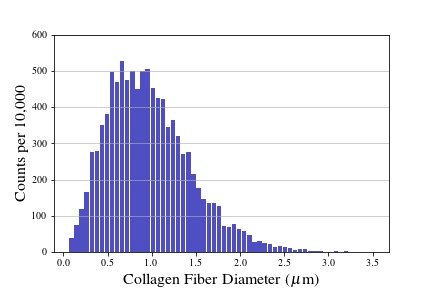
\includegraphics[width=0.45\textwidth]{figures/collagenFiberDiaHistogram.jpg}
    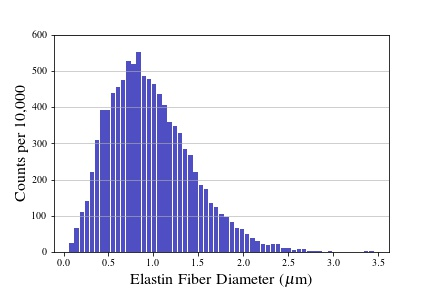
\includegraphics[width=0.45\textwidth]{figures/elastinFiberDiaHistogram.jpg}
    \caption{Typical histograms for collagen and elastin chord diameters pertaining to the statistics reported in Table~\ref{tab:alveolarProp}.  Their tails weigh heavy at the larger diameters, because their distributions are normal in the square root of their diameters.  These histograms are identical, for all practical purposes.}
    \label{fig:septalChordStats}
\end{figure}

The collagen and elastin fibers that make up a septal chord have the same length, they experience the same strain, and they exist at the same temperature; therefore, we employ Eqn.~(\ref{Helmholtz1D}) as the governing constitutive equation to describe their mechanical behavior
\begin{displaymath}
\left\{ \begin{matrix} 
\mathrm{d} \eta \\ \mathrm{d} s
\end{matrix} \right\} = \begin{bmatrix}
C / \theta - E \alpha^2 / \rho & E \alpha / \rho \\
-E  \alpha & E
\end{bmatrix} \left\{ \begin{matrix}
\mathrm{d} \theta \\ \mathrm{d} e
\end{matrix} \right\} 
\end{displaymath}
wherein $\eta$ is the entropy density (erg/gr.K) and $s$ is the chordal stress (barye = $\text{dyne/cm}^2$) in an engineering sense (force per unit reference area) with material constants: $C$ is a specific heat at constant pressure (erg/gr.K), $\alpha$ is a linear coefficient of thermal expansion (1/K), $E$ is an elastic modulus ($\text{dyne/cm}^2$ = $\text{erg/cm}^3$), and $\rho$ is its mass density ($\text{gr/cm}^3$).  Because $\mathrm{d} \theta = 0$ across a wave front \cite{AmesStaff53}, this general system reduces to
\begin{displaymath} 
\mathrm{d} s = E \, \mathrm{d}e
\quad \text{and} \quad
\rho \, \mathrm{d} \eta = E \alpha \, \mathrm{d}e
\end{displaymath} 
wherein the first equation establishes a change in stress carried by a chord, while the second equation establishes a change in entropy per unit volume of chord. 

\subsubsection{Chordal Forces and Entropies}

The constitutive equations that govern alveolar chords, suitable for studying shock waves in lungs, are described by the following equations
\begin{subequations}
    \label{septalChordCEs}
    \begin{align}
    F^f & = s^c A^c + s^e A^e &
    \mathrm{d} s^c & = E^c ( e, s^c ) \, \mathrm{d}e & 
    \mathrm{d} s^e & = E^e ( e, s^e ) \, \mathrm{d}e \\
    S^f & = S^c + S^e & 
    S^c & = S_0^c + \alpha^c s^c V^c & 
    S^e & = S_0^e + \alpha^e s^e V^e
    \end{align}
\end{subequations}  
wherein $F^f$ (dyne) is the fiber force carried by a septal chord, with $s^c$ and $s^e$ being the engineering stresses carried by its collagen and elastin fibers that when multiplied by their reference cross-sectional areas $A^c$ and $A^e$ gives rise to the forces they carry.  Variable $S^f$ (erg/K) denotes the fiber entropy of a septal chord, with $S^c$ and $S^e$ being the entropies of its two parts.  For initial conditions, let $s^c_0 = s^c |_{L = L_0} = 0$ and $s^e_0 = s^e |_{L = L_0} = 0$, and let $S_0^c = \rho^c V^c \eta^c$ and $S_0^e = \rho^e V^e \eta^e$, wherein $\rho^c$ and $\rho^e$ are the mass densities, which are constant because their volumes $V^c$ and $V^e$ are taken to be conserved, while $\eta^c$ and $\eta^e$ are the entropy densities at rest.  It remains to establish the two tangent moduli $E^c (e, s^c)$ and $E^e (e, s^e)$ for collagen and elastin.  These tangent moduli are considered to be implicit functions of state in our modeling of alveolar chords below, see e.g., Ref.~\cite{FreedRajagopal16}.

Collagen is a fiber comprised of numerous, long, slender, wavy filaments whose waviness, known as crimp, straightens under sufficient deformation \cite{Kastelicetal'78,FreedDoehring05}.  Elastin is a linked fiber network, much like an elastomer, whose filaments between crosslinks rotate to align with an axis of loading under sufficient deformation \cite{AaronGosline81,Urry89}.  Consequently, collagen and elastin both recruit constituent filaments with increasing deformation into an overall, load-bearing, fiber response.  The internal energies of collagen and elastin may therefore be thought of as being comprised of a configurational energy and a strain energy.  As such, both collagen and elastin are modeled as Freed-Rajagopal biologic fibers, which are described in terms of two such energies.  Their model is derived from the theory of implicit elasticity in \ref{appImplicitElasticity}.  According to their model, tangent compliances for collagen and elastin are described by
\begin{subequations}
    \label{septalChordModuli}
    \begin{align}
	\frac{1}{E^c (\theta, e, s^c)} & = \frac{e_t^c - e_1^c}{E_1^c e_t^c + 2s^c} + \frac{1}{E_2^c} &
	e_1^c & = e - \alpha^c (\theta - \theta_0) - \frac{s^c}{E_2^c} \\
    \frac{1}{E^e (\theta , e , s^e )} & = \frac{e_t^e - e_1^e}{E_1^e e_t^e + 2s^e} + \frac{1}{E_2^e} &
    e_1^e & = e - \alpha^e (\theta - \theta_0) - \frac{s^e}{E_2^e} 
    \end{align}
\end{subequations}
where material constants $E_1^c$ and $E_2^c$ are two asymptotic moduli for collagen bounding the response, i.e., $E_1^c \leq E^c \leq E^c_2$, while $E_1^e$ and $E_2^e$ are two asymptotic moduli for elastin bounding its response, viz., $E^e_1 \leq E^e \leq E^e_2$, all of which here have units of stress (barye = dyne/$\text{cm}^2$), with $e_t^c$ and $e_t^e$ being their respective transition strains, cf.\ \ref{appImplicitElasticity}. 

The material properties needed to model septal chords are listed in Tables~\ref{tab:alveolarProp} \& \ref{tableCollagenElastin}.  From Eqn.~(\ref{thermodynamicConstraints}), these moduli are bound from above by $E^c_{\max} = 4.9 \times 10^9$~barye ($\text{dyne/cm}^2$) and $E^e_{\max} = 1.7 \times 10^9$~barye.  We therefore observe that $E^c_2$ and $E^e_2$ are about 100 times smaller than $E^c_{\max}$ and $E^e_{\max}$.  We recall that $\theta = \theta_0$ in our application, so the $e^c_1$ and $e^e_1$ strains defined in the second column above simplify somewhat.  

\begin{table}
    \centering
    \begin{tabular}{|l|l|l|}
        \hline
        \multicolumn{3}{|c|}{Collagen$\vphantom{|^{|^|}}$} \\ \hline
        $\rho^c$ \hfill [$\textrm{gr/cm}^{3^{\phantom{|}}}$] & $1.34$ & 
        Fels \cite{Fels64} \\
        $\eta^c$ \hfill [erg/gr.K] & $3.7 \times 10^7$ &  \\
        $C^c$ \hfill [erg/gr.K] & $1.7 \times 10^7$ & 
        Kanagy \cite{Kanagy55} \\
        $\alpha^c$ \hfill [1/C] & $1.8 \times 10^{-4}$ & 
        Weir \cite{Weir48}  \\
        $e^c_t$ & $0.09$ & estimated from TLC $\approx$ 30\% \\
        $E_1^c$ \hfill [barye] & $5.0 \times 10^5$ &  \\
        $E_2^c$ \hfill [barye] & $3.0 \times 10^7$ &  \\ \hline
        \multicolumn{3}{|c|}{Elastin$\vphantom{|^{|^|}}$} \\ \hline 
        Parameter & Value & Reference \\ \hline
        $\rho^e$ \hfill [$\textrm{gr/cm}^{3^{\phantom{|}}}$] & $1.31$ & 
        Lillie \& Gosline \cite{LillieGosline02a} \\
        $\eta^e$ \hfill [erg/gr.K] & $3.4 \times 10^7$ & 
        Shadwick \& Gosline \cite{ShadwickGosline85} \\
        $C^e$ \hfill [$\textrm{erg/gr.K}$] & $4.2 \times 10^7$  & 
        Kakivaya \& Hoeve \cite{KakivayaHoeve75} \\
        $\alpha^e$ \hfill [1/C] & $3.2\times 10^{-4}$ & 
        Lillie \& Gosline \cite{LillieGosline02a} \\ 
        $e^e_t$ & 0.4 & Shadwick \& Gosline \cite{ShadwickGosline85} \\
        $E^e_1$ \hfill [barye] & $2.3 \times 10^6$ & Urry \cite[Fig.~18]{Urry89} \\ 
        $E^e_2$ \hfill [barye] & $1.0 \times 10^7$ & 
        Lillie \& Gosline \cite[Fig.~5]{LillieGosline07} \\ \hline
    \end{tabular}
    \caption{Physical properties for hydrated collagen and elastin fibers.  Collagen denatures at around $60^\circ$C \cite{HoermannSchlebusch71}, i.e., above this temperature collagen will shrink rapidly---an effect not modeled here.}
    \label{tableCollagenElastin}
\end{table}

The actual force and entropy carried by an individual septal chord in our alveolar model will be one third of their calculated values from Eqn.~(\ref{septalChordCEs}), because each chord is typically shared between three neighboring alveoli.

\subsection{Conjugate Pairs $\Longleftrightarrow$ Tensor Components for a Membrane}
\label{secConjugatePairs}

The above planar strains and their rates are defined accordingly \cite{Freedetal17}
\begin{subequations}
    \label{conjugateStrains}
    \begin{align}
    \xi & \defeq \ln \sqrt{\frac{a}{a_0} \frac{b}{b_0}} = 
    \ln \sqrt{\frac{A}{A_0}} &
    \varepsilon & \defeq \ln \sqrt{\frac{b_0}{a_0} \frac{a}{b}} = 
    \ln \sqrt{\frac{\Gamma}{\Gamma_0}} &
    \gamma & \defeq g - g_0 \label{thermoStrains3} \\
    \mathrm{d} \xi & \hspace{2.5pt} = \frac{1}{2} 
    \left( \frac{\mathrm{d} a}{a} + \frac{\mathrm{d} b}{b} \right) = 
    \frac{1}{2} \frac{\mathrm{d} A}{A} &
    \mathrm{d} \varepsilon & \hspace{2.5pt} = \frac{1}{2} 
    \left( \frac{\mathrm{d}a}{a} - \frac{\mathrm{d}b}{b} \right) = 
    \frac{1}{2} \frac{\mathrm{d} \Gamma}{\Gamma} & 
    \mathrm{d} \gamma & \hspace{2.5pt} = \mathrm{d} g
    \label{thermoStrainRates3} 
    \end{align}
\end{subequations}
where $a, b, g$ are the physical attributes illustrated in Fig.~\ref{figKinematics}, with $a_0 , b_0 , g_0$ being their reference values, which are selected so that $\xi_0 = \varepsilon_0 = \gamma_0 = 0$, as established in Part~\ref{partKinematics} via a Gram-Schmidt factorization of the deformation gradient.  These strains are two-state fields, independent of path---a tacit requirement of thermo\-dynamics \cite{Caratheodory09}.  We point out that $\xi = \ln \sqrt{A / A_0}$ where $A = ab$ denotes area, and $\varepsilon = \ln \sqrt{\Gamma / \Gamma_0}$ where $\Gamma = a/b$ denotes the stretch of squeeze, i.e., the stretch of a pure shear deformation is in the sense of Becker \cite{Becker93} and Treloar \cite{Treloar75}. Thermo\-dynamic strains $\xi , \varepsilon , \gamma$ and their differential rates $\mathrm{d} \xi , \mathrm{d} \varepsilon , \mathrm{d} \gamma$ are exported by class \texttt{pentagon} according to Freed \& Zamani \cite{FreedZamani18}, cf.\ \ref{appPentagons}.

The conjugate stresses to the above planar strains are determined to be
\begin{subequations}
    \label{conjugateStresses}
    \begin{align}
    \pi & \defeq \frac{\pi}{w} = \mathcal{S}_{11} + \mathcal{S}_{22} & 
    s^{\sigma} & \defeq \frac{\sigma}{w} = \mathcal{S}_{11} - \mathcal{S}_{22} & 
    s^{\tau} & \defeq \frac{\tau}{w} = \Gamma \mathcal{S}_{21}
    \label{thermoStresses3} \\
    \intertext{which follow from Eqns.~(\ref{convectedWorkRate} \& \ref{thermoStrainRates3}).  Here $w$ denotes a reference width or thickness of a membrane, i.e., $\pi$, $s^{\sigma}$ and $s^{\tau}$ are engineering stresses.  Consequently, components $\mathcal{S}_{ij}$ now have units of stress ($\text{dyne/cm}^2$) instead of surface tension (dyne/cm).  Conversely, the physical components of stress $\mathcal{S}_{ij}$ are established through}
    \mathcal{S}_{11} & = \tfrac{1}{2} ( s^{\pi} + s^{\sigma} ) &
    \mathcal{S}_{22} & = \tfrac{1}{2}( s^{\pi} - s^{\sigma} ) &
    \mathcal{S}_{12} & = \mathcal{S}_{21} = s^{\tau}  / \, \Gamma
    \label{stresses3}
    \end{align}
\end{subequations} 
when described in terms of their thermo\-dynamic attributes $s^{\pi}$, $s^{\sigma}$ and $s^{\tau}$, plus the squeeze stretch $\Gamma$ that must appear in $s^{\tau}$ so that $\mathrm{d} \gamma$ associates with an exact differential.  The coupling appearing in the definition for shear stress, viz., $\Gamma \mathcal{S}_{21}$, is the reason why a coupling exists between squeeze and shear in constitutive equation~(\ref{HelmholtzMembraneODEs}).

The stress $\boldsymbol{\mathcal{S}}$ occurring in a septal plane, when evaluated in a pentagonal co-ordinate frame $( \vec{\mathbfit{e}}_{\hspace{0.5pt}1} , \vec{\mathbfit{e}}_{\hspace{0.5pt}2} , \vec{\mathbfit{e}}_{\hspace{0.5pt}3} )$, has non-zero components in the plane, i.e., in the upper-left $2 \times 2$ sub-matrix, with the alveolar pressure $P$ supplying $\mathcal{S}_{33} = -P$.  These components map into a Kirchhoff stress $\mathbf{s}$ expressed in the dodecahedral frame of reference $( \vec{\boldsymbol{\imath}} , \vec{\boldsymbol{\jmath}} , \vec{\mathbfit{k}} )$ via a component transformation of $s_{ij} = P_{ik} Q_{k\ell} \mathcal{R}_{\ell m} \mathcal{S}_{mn} \mathcal{R}_{on} Q_{po} P_{jp}$.   Because $s_{12} = s_{21}$, and because $\mathbf{P}$, $\mathbf{Q}$ and $\boldsymbol{\mathcal{R}}$ are each orthogonal tensors, it necessarily follows that $\mathcal{S}_{12} = \mathcal{S}_{21}$.  Matrix $\mathbf{P}$ is a rotation of the pentagonal frame of reference about that of the dodecahedron's axes, matrix $\mathbf{Q}$ is a rotation for re-indexing pentagonal co-ordinates, and matrix $\boldsymbol{\mathcal{R}}$ is a Gram-Schmidt rotation.

\subsubsection{Modeling an Alveolar Membrane Subjected to a Shock Wave}
  
From a mechanics perspective, we know a great deal more about alveolar chords than we know about alveolar septa.  More judgment will therefore be required in our construction and parameterization of a material model for alveolar membranes.  

A typical alveolar septum is 4-5 $\mu$m in width \cite{Sukietal11}.  They are comprised of an outside layer of epithelial cells that encase capillaries made of endothelial cells along with a basement membrane that is composed of unorganized collagen and elastin filaments, plus proteoglycans and other extracellular proteins.  This basement membrane, roughly at mid-plane in an alveolar septum, has a width of about $0.5 \, \mu$m \cite{RoanWaters11}.  Inertial forces generated by these membranes are to be based upon a membrane thickness of $\sim\!\!5$~$\mu$m with an approximate density of water, while the structural forces that they carry are to be based upon a basement membrane thickness of $\sim\!\! 0.5$~$\mu$m.  

It is not known how much of the mechanical load is actually carried by the cells in an alveolar septum vs.\ the extracellular basement membrane they encase, but it is generally thought that this basement membrane carries the majority of the load \cite{Sukietal11}.  Therefore, by diminishing the moduli that are appropriate for describing a basement membrane with thickness $\sim\!\! 0.5$~$\mu$m by a factor of 10, we get estimates for effective septal moduli that are applicable when modeling a whole septal membrane with thickness $\sim\!\! 5$~$\mu$m.  We use the model parameters obtained for a visceral pleura membrane \cite{Freedetal17} and the above conjecture to model alveolar septa.

From Eqns.~(\ref{HelmholtzMembraneODEsB} \& \ref{conjugateStresses}), alveolar septa are determined to have a constitutive response that, in the presence of shock waves, are governed by
\begin{subequations}
    \begin{align}
\left\{ \begin{matrix}
\mathrm{d} s^{\pi} \\ \mathrm{d} s^{\sigma} \\ \mathrm{d} s^{\tau}
\end{matrix} \right\} & = \begin{bmatrix}
4 M & 0 & 0 \\
0 & 2 N & 2 s^{\tau} \\
0 & 2 s^{\tau} & G
\end{bmatrix} \left\{ \begin{matrix}
\mathrm{d} \xi \\ \mathrm{d} \varepsilon \\ \mathrm{d} \gamma
\end{matrix} \right\} \\
\intertext{that when integrated produce a rotated Kirchhoff stress located at a Gauss point belonging to a pentagon of interest with components}
\begin{bmatrix} 
\mathcal{S}_{11} & \mathcal{S}_{12} & \mathcal{S}_{13} \\
\mathcal{S}_{21} & \mathcal{S}_{22} & \mathcal{S}_{23} \\
\mathcal{S}_{31} & \mathcal{S}_{32} & \mathcal{S}_{33}
\end{bmatrix} & = \begin{bmatrix}
\tfrac{1}{2} ( s^{\pi} + s^{\sigma} ) & b \hspace{0.5pt} s^{\tau} / a & 0 \\
b \hspace{0.5pt} s^{\tau} / a & \tfrac{1}{2} ( s^{\pi} - s^{\sigma} ) & 0 \\
0 & 0 & -P
\end{bmatrix} \label{septalStresses} \\
\intertext{along with a septal (membrane) entropy of}
S^m & = S^m_0 + 2 \alpha s^{\pi} V^m
\end{align}
\end{subequations}
where $S^m$ (erg/K) describes the entropy of a membrane with $S_0^m = \rho^m V^m \eta^m$ denoting its entropy at rest, wherein $\rho^m$ is its mass density, which is constant because its volume $V^m$ is taken to be conserved, and $\eta^m$ is the entropy density at rest, while $\alpha$ is the coefficient of linear thermal expansion, which is twice that of the areal expansion coefficient.  Material constant $M(\xi, s^{\pi})$ is the dilation modulus, $N(\varepsilon, s^{\sigma})$ is the squeeze modulus, and $G(\gamma, s^{\tau})$ is the shear modulus.  All moduli now have units of stress.

Collagen and elastin appear as thin filaments randomly oriented and somewhat uniformly dispersed throughout a basement membrane, unlike the strongly aligned fibers that appear in septal chords.  Consequently, for our purposes, we model this collective ensemble of tissue and structure types as a homo\-geneous isotropic membrane modeled after the Freed-Rajagopal biologic fiber \cite{FreedRajagopal16} that we have extended to membranes in \ref{appImplicitElasticity}, specifically
\begin{subequations}
    \label{septalCompliances}
    \begin{align}
    \frac{1}{M} & = \frac{\xi_t - \xi_1}{M_1 \xi_t + s^{\pi} / 2} + \frac{1}{M_2} &
    \xi_1 & = \xi - \alpha ( \theta - \theta_0 ) - \frac{s^{\pi}}{4M_2}
    \label{septalDilationCompliance} \\
    \frac{1}{N} & = 2 \left( \frac{ \varepsilon_t - | \varepsilon_1 |}{N_1 \varepsilon_t + 2 \gamma s^{\tau}} + \frac{1}{N_2} \right) & 
    \varepsilon_1 & = \varepsilon - \frac{s^{\sigma} - 2 \gamma s^{\tau}}{N_2}
    \label{septalSqueezeCompliance} \\
    \frac{1}{G} & = \Gamma \left( \frac{\gamma_t - 2\varepsilon \gamma - | \gamma_1 |}{G_1 \gamma_t + 2 \varepsilon s^{\tau}} + \frac{1-2\varepsilon}{G_2} \right) & 
    \gamma_1 & = \gamma - \frac{(1 - 2\varepsilon) s^{\tau}}{G_2}
    \label{septalShearCompliance}
    \end{align}
\end{subequations}
where the compliant tangent moduli of $M_1, N_1$ and $G_1$ and the stiff, terminal, tangent moduli of $M_2 , N_2$ and $G_2$ bound their responses in that $M_1 \leq M \leq M_2$, $N_1 \leq N \leq N_2$ and $G_1 \leq G \leq G_2$, with gradual transitions between their asymptotic bounds being centered around strains of $\xi_t , \varepsilon_t$ and $\gamma_t$.

Finite element technology is used to interpolate these stresses to forces at the vertices of a pentagon, cf.\ Part~\ref{partVariational}.  The stress components that actually get interpolated to the element nodes follow from a mapping of $\mathbf{Q} \boldsymbol{\mathcal{RSR}}^{\mathsf{T}} \mathbf{Q}^{\mathsf{T}}$, where $\boldsymbol{\mathcal{R}}$ is the orthogonal rotation coming from the \textbf{QR} decomposition of a deformation gradient, and where $\mathbf{Q}$ is the matrix that re-indexes the co-ordinate indices.  The actual forces and entropy interpolated to these nodes are halved, because each septal plane belongs to two neighboring alveoli. 

\subsection{Modeling an Alveolar Volume Subjected to a Shock Wave}
\label{sec:IdealGasLaw}

Alveoli are connected to bronchial trees via alveolar ducts.  Under normal conditions, air moves in and out of the alveoli via these ducts.  However, when subjected to a stress wave passing over an alveolus, there is no time for the transport of air to take place.  Hence, we can consider the air (and heat) within an alveolus to become `trapped', and the pressure to be uniform therein.  The governing process is therefore adiabatic.  It is under this condition that we model the volumetric response of alveolar sacs.

If one considers the saturated air\slash fluid within an alveolus to be an ideal gas, then \cite{Davison08}
\begin{equation}
P V = n \! R \theta
\quad \text{or} \quad
\frac{P V}{\theta} = \frac{P_0 V_0}{\theta_0} = n \! R = \mathrm{constant}
\label{idealGas}
\end{equation}
where, in our case, $P_0$ is taken to be atmospheric pressure at sea level (1~bar or $10^5$~Pa or $10^6$~barye), with $V_0$ being that alveolar volume whereat alveolar pressure and plural pressure are both atmospheric, while $\theta_0 = 37^{\circ}$C = 310~K is assigned as body temperature.  Parameter $n$ is the molar content of gas within an alveolus, with $R$  being the universal gas constant.  

The material constants associated with an ideal gas contained within an adiabatic enclosure are
\begin{equation}
\alpha \defeq \frac{1}{V} \left. \frac{\partial V}{\partial \theta} \right|_P = 
\frac{1}{\theta_0} \, \frac{P_0 V_0}{P V}
\quad \text{and} \quad
K \defeq -\frac{1}{V} \left. \frac{\partial P}{\partial V} \right|_{\theta} = 
P_0 \, \frac{V_0 \hspace{0.5pt} \theta}{\theta_0 V}
\label{idealGasConstants}
\end{equation}
with the other two material constants pertaining to moist air at body temperature\footnote{
    The physical properties listed for air were taken from the website \texttt{www.peacesoftware.de} hosted by Berndt Wischnewski.
}
being its mass density $\rho$ of $1.125 \times 10^{-3} \; \text{gr/cm}^3$ and its specific heat $C$ at constant pressure of $1.007 \times 10^7$~erg/gr.K, constrained by the fact that $K < K_{\max} = \rho C / \alpha^2 \theta \approx \rho C \theta$.

An alveolar sac is modeled as an adiabatic pressure vessel filled with an ideal gas whose Helmholtz formulation (\ref{Helmholtz3D}) is described by
\begin{equation}
\left\{ \begin{matrix}
\rho \, \mathrm{d} \eta \\ -3 \, \mathrm{d} P
\end{matrix} \right\} = \begin{bmatrix}
\rho C / \theta - K \alpha^2 & 3 K \alpha \\ 
-3K\alpha & 9K
\end{bmatrix} \left\{ \begin{matrix}
\mathrm{d} \theta \\ \mathrm{d} \Xi
\end{matrix} \right\}
\label{alveolarGas}
\end{equation}
that, again, because $\theta = \theta_0$ across a wave front \cite{AmesStaff53}, simplifies the governing system of differential equations (\ref{alveolarGas}) to
\begin{displaymath}
    \mathrm{d}P = -3K \, \mathrm{d} \Xi 
    \quad \text{and} \quad
    \rho \, \mathrm{d} \eta = 3 K \alpha \, \mathrm{d} \Xi
\end{displaymath}
where we recall that $\mathrm{d}\Xi = \tfrac{1}{3} V^{-1} \, \mathrm{d} V$.  Like before, we do not want the entropy per unit mass or per unit volume; rather, we prefer to know what the entropy of its structural constituent is, in this case, the gas within an alveolar sac.  To find this, we multiply the right-hand expression through by volume $V_0$, after which we integrate both differential equations to get
\begin{equation}
    \frac{P}{P_0} = \frac{V_0}{V}
    \quad \therefore \quad
    \alpha = \frac{1}{\theta_0}
    \quad \implies \quad
    S^a = S^a_0 + \frac{V_0 ( P_0 - P )}{\theta_0}
    \label{alveolarSacCE}
\end{equation}
where $S^a$ is the desired entropy of the air within an alveolar sac with $S^a_0 = \rho^a V^a_0 \eta^a$ given that $\rho^a \eta^a$ is the entropy per unit volume of humid air at body temperature and atmospheric pressure, viz., $\rho^a \eta^a = 7.770 \times 10^4 \: \text{erg/cm}^3\text{.K}$.  The above results are in agreement with the ideal gas law, as they should be, because $\alpha$ and $K$ in Eqn.~(\ref{idealGasConstants}) were both derived from this law.

Pressure $P$ is mapped to nodal forces at the vertices of a dodecahedron via Eqn.~(\ref{septalStresses}) in our alveolar model.  This requires finite element technology, which is discussed in Part~\ref{partVariational}.

\section{Finite Element Implementation of Constitutive Equations}
\label{secFE_CE}

These constitutive models are implemented into our finite element model as hypo\-elastic material models \cite{Truesdell55} described by\footnote{
    At present, the tangent modulus $\boldsymbol{M}$ is not considered to have an explicit dependence upon time.  In other words, visco\-elastic phenomena cannot be accounted for in the current formulation.
}
\begin{equation}
\dot{\boldsymbol{\sigma}} = \mathbf{M} \bigl( \boldsymbol{\sigma}, \boldsymbol{\epsilon} ( \boldsymbol{\lambda} ) \bigr) \, \dot{\boldsymbol{\epsilon}} 
\quad \text{or equivalently} \quad
\dot{\boldsymbol{\sigma}} = 
\mathbf{M} \bigl( \boldsymbol{\sigma} , \boldsymbol{\epsilon} ( \boldsymbol{\lambda} ) \bigr) \, \frac{\mathrm{d} \boldsymbol{\epsilon}}
{\mathrm{d} \boldsymbol{\lambda}} \, \dot{\boldsymbol{\lambda}}
\end{equation}
where $\boldsymbol{\sigma}$, $\boldsymbol{\epsilon}$ and $\boldsymbol{\lambda}$ are arrays of stress, strain and stretch attributes, respectively, with matrix $\mathbf{M} ( \boldsymbol{\sigma}, \boldsymbol{\epsilon} )$ containing the tangent moduli, i.e., $\mathrm{d} \boldsymbol{\sigma} / \mathrm{d} \boldsymbol{\epsilon}$, that, in general, depend upon the currents states of stress $\boldsymbol{\sigma}$ and strain $\boldsymbol{\epsilon}$, with strain in turn depending upon stretch $\boldsymbol{\lambda}$.  The above constitutive equation is actually integrated for the stress attributes $\boldsymbol{\sigma}$ in the finite element equations themselves.

The strain attributes, either $\boldsymbol{\epsilon}_{2D} ( \boldsymbol{\lambda}_{2D} )$ whereby $\boldsymbol{\lambda}_{2D} = \{ \theta , a , b , \gamma \}^{\mathsf{T}}$ or $\boldsymbol{\epsilon}_{3D} ( \boldsymbol{\lambda}_{3D} )$ whereby $\boldsymbol{\lambda}_{3D} = \{ \theta , a , b , c , \alpha , \beta , \gamma \}^{\mathsf{T}}$, as appropriate, have elements comprised of temperature $\theta$ and a set of physical stretches extracted from the components of Laplace stretch $\boldsymbol{U}$ via
\begin{equation}
\boldsymbol{U}_{2D} = 
\begin{bmatrix} 
a & a \gamma \\ 0 & b 
\end{bmatrix}
\quad \text{and} \quad 
\boldsymbol{U}_{3D} = 
\begin{bmatrix}
a & a \gamma & a \beta \\ 0 & b & b \alpha \\ 0 & 0 & c
\end{bmatrix}
\label{LaplaceStretch}
\end{equation}
with components $U_{ij}$ evaluated according to the formul\ae\
\begin{equation}
\begin{aligned}
U_{11} & = \sqrt{C_{11}} & 
U_{12} & = C_{12} / U_{11} &
U_{13} & = C_{13} / U_{11} \\
U_{21} & = 0 &
U_{22} & = \sqrt{C_{22} - U_{12}^{\,2}} &
U_{23} & = \bigl( C_{23} - U_{12\,}U_{13} \bigr) / U_{22} \\
U_{31} & = 0 &
U_{32} & = 0 & 
U_{33} & = \sqrt{C_{33} - U_{13}^{\,2} - U_{23}^{\,2}}
\end{aligned}
\label{LagrangianLaplaceStretch}
\end{equation}
so that
\begin{equation}
a \defeq U_{11} , \quad
b \defeq U_{22} , \quad
c \defeq U_{33} , \quad
\alpha \defeq \frac{U_{23}}{U_{22}} , \quad
\beta \defeq \frac{U_{13}}{U_{11}} , \quad
\gamma \defeq \frac{U_{12}}{U_{11}}
\label{LagrangianPhysicalAttributes}
\end{equation}
wherein $\mathbf{C} = \mathbf{F}^{\mathsf{F}} \mathbf{F}$ is the right Cauchy-Green deformation tensor.  Attributes $a$, $b$ and $c$ are elongation ratios, while attributes $\alpha$, $\beta$ and $\gamma$ are extents of shear. Components for $\boldsymbol{U}_{2D}$ associate with the upper-left $2 \! \times \! 2$ submatrix of the above matrix elements. 

\subsection{Thermodynamic Strains}

In 2D, the strain attributes $\boldsymbol{\epsilon}_{2D}  = \{ \theta , \xi , \varepsilon , \gamma \}^{\mathsf{T}}$ that are used in our analysis are given by
\begin{subequations}
    \label{thermodynamicStrains}
    \begin{align}
    \xi & = \ln \left( \sqrt{\frac{ab}{a_0 b_0}} \right) &
    \varepsilon & = \ln \left( \sqrt{ \frac{a}{a_0} \frac{b_0}{b} } \right) &
    \gamma & = \gamma - \gamma_0 \\
    \intertext{where $\theta$ denotes temperature, $\xi$ denotes dilation, $\varepsilon$ denotes pure shear, and $\gamma$ denotes simple shear.  In 3D, the strain attributes $\boldsymbol{\epsilon}_{3D} = \{ \theta , \Xi , \varepsilon_1 , \varepsilon_2 , \gamma_1 , \gamma_2 , \gamma_3  \}^{\mathsf{T}}$ become}
    \Xi & = \ln \left( \sqrt[3]{\frac{abc}{a_0 b_0 c_0}} \right) &
    \varepsilon_1 & = \ln \left( \sqrt[3]{\frac{a}{a_0} \frac{b_0}{b}} \right) &
    \varepsilon_2 & = \ln \left( \sqrt[3]{\frac{b}{b_0} \frac{c_0}{c}} \right) \notag \\
    \gamma_1 & = \alpha - \alpha_0 &
    \gamma_2 & = \beta - \beta_0 &
    \gamma_3 & = \gamma - \gamma_0
    \end{align}
\end{subequations}
where $\theta$ denotes temperature, $\Xi$ denotes dilatation, $\varepsilon_1$ denotes a squeeze in the 12~plane, $\varepsilon_2$ denotes a squeeze in the 23-plane, while $\gamma_1$, $\gamma_2$ and $\gamma_3$ are three orthogonal simple shears.  From these definitions for thermo\-dynamic strains, one determines that
\begin{subequations}
    \label{strainGradient}
    \begin{align}
    \left\{ \begin{matrix}
    \dot{\theta} \\ \dot{\xi} \\ \dot{\varepsilon} \\ \dot{\gamma}
    \end{matrix} \right\} & = \begin{bmatrix}
    1 & 0 & 0 & 0 \\ 0 & 1/2a & 1/2b & 0 \\ 0 & 1/2a & -1/2b & 0 \\ 0 & 0 & 0 & 1
    \end{bmatrix} \left\{ \begin{matrix}
    \dot{\theta} \\ \dot{a} \\ \dot{b} \\ \dot{\gamma}
    \end{matrix} \right\} \\
    \intertext{and}
    \left\{ \begin{matrix}
    \dot{\theta} \\ \dot{\Xi} \\ \dot{\varepsilon}_1 \\ \dot{\varepsilon}_2 \\ 
    \dot{\gamma}_1 \\ \dot{\gamma}_2 \\ \dot{\gamma}_3
    \end{matrix} \right\} & = \begin{bmatrix}
    1 & 0 & 0 & 0 & 0 & 0 & 0 \\
    0 & 1/3a & 1/3b & 1/3c & 0 & 0 & 0 \\ 
    0 & 1/3a & -1/3b & 0 & 0 & 0 & 0 \\ 
    0 & 0 & 1/3b & -1/3c & 0 & 0 & 0 \\
    0 & 0 & 0 & 0 & 1 & 0 & 0 \\
    0 & 0 & 0 & 0 & 0 & 1 & 0 \\
    0 & 0 & 0 & 0 & 0 & 0 & 1
    \end{bmatrix} \left\{ \begin{matrix}
    \dot{\theta} \\ \dot{a} \\ \dot{b} \\ \dot{c} \\ 
    \dot{\alpha} \\ \dot{\beta} \\ \dot{\gamma}
    \end{matrix} \right\}
    \end{align}
\end{subequations}
where we see that the matrices $\mathrm{d} \boldsymbol{\epsilon} / \mathrm{d} \boldsymbol{\lambda}$ depend upon elongations $a$, $b$ and, in the 3D case, $c$.

\subsection{Stretch Rates}

The following approximations for stretch rates $\{ \dot{a} , \dot{b} , \dot{\gamma} \}^{\mathsf{T}}$ and $\{ \dot{a} , \dot{b} , \dot{c} , \dot{\alpha} , \dot{\beta} , \dot{\gamma} \}^{\mathsf{T}}$ were derived by Freed \&\ Zamani \cite{FreedZamani18}.  They populate the right-hand vectors in Eqn.~(\ref{strainGradient}).

A forward difference formula is used to approximate rates for the various stretch attributes, as obtained from $\dot{\boldsymbol{U}}_0 = ( \boldsymbol{U}_1 -  \boldsymbol{U}_0 ) / h + \mathcal{O}(h)$, thereby resulting in the following formul\ae\
\begin{equation}
\begin{aligned}
\dot{a}_0 &
\approx \frac {a_1 - a_0}{h} \quad &
\dot{\alpha}_0 & 
\approx \frac{b_1}{b_0} \left(\frac{\alpha_1 - \alpha_0}{h} \right) \\
\dot{b}_0 & 
\approx \frac {b_1 - b_0}{h} \quad & 
\dot{\beta}_0 & 
\approx \frac{a_1}{a_0} \left( \frac{\beta_1 - \beta_0}{h} \right) \\
\dot{c}_0 & 
\approx \frac {c_1 - c_0}{h} \quad & 
\dot{\gamma}_0 & \approx \frac{a_1}{a_0} \left( \frac{\gamma_1 - \gamma_0}{h}\right)
\end{aligned}
\label{forwardDifference1stOrder}
\end{equation}
while a backward difference formula $\dot{\boldsymbol{U}}_1 = ( \boldsymbol{U}_1 -  \boldsymbol{U}_0 ) / h + \mathcal{O}(h)$ is used to estimate rates for the various stretch attributes at the end of its first integration step, from which it follows that
\begin{equation}
\begin{aligned}
\dot{a}_1 & 
\approx \frac {a_1 - a_0}{h} \;\; & 
\dot{\alpha}_1 & 
\approx \frac {b_0}{b_1} \left( \frac{\alpha_1 - \alpha_0}{h} \right) \\
\dot{b}_1 & 
\approx \frac {b_1 - b_0}{h} \;\; & 
\dot{\beta}_1 & 
\approx \frac {a_0} {a_1} \left( \frac{\beta_1 - \beta_0}{h} \right) \\
\dot{c}_1 & 
\approx \frac {c_1 - c_0}{h} \;\; & 
\dot{\gamma}_1 & 
\approx \frac{a_0}{a_1} \left(\frac{\gamma_1 - \gamma_0}{h} \right)
\end{aligned}
\label{backwardDifference1stOrder}
\end{equation}
with there being a distinction in how the shear rates are approximated at the end points of this first interval of integration.  2D is an obvious special case of 3D.

Equations (\ref{forwardDifference1stOrder} \& \ref{backwardDifference1stOrder}) are first-order approximations for these derivatives.  Second-order approximations can be established whenever $n > 0$ provided the stepsize for step $[n, n+1]$ equals the stepsize for step $[n-1, n]$, where state $n=0$ associates with an initial condition.  The backward difference formula  $\dot{\boldsymbol{U}}_{n+1} = ( 3 \, \boldsymbol{U}_{n+1} -  4 \, \boldsymbol{U}_{n} + \boldsymbol{U}_{n-1} ) / 2h + \mathcal{O}(h^2)$ produces stretch rates of
\begin{equation}
\begin{aligned}
\dot{a}_{n+1} & 
\approx \frac {3a_{n+1} - 4a_{n} +  a_{n-1}}{2h} \\ 
\dot{b}_{n+1} & 
\approx \frac {3b_{n+1} - 4b_{n} +  b_{n-1}}{2h} \\
\dot{c}_{n+1} & 
\approx \frac {3c_{n+1} - 4c_{n} +  c_{n-1}}{2h} \\
\dot{\alpha}_{n+1} & 
\approx \frac{2b_{n}} {b_{n+1}} \left( \frac{\alpha_{n+1} - \alpha_{n}}{h} \right) - \frac{b_{n-1}} {b_{n+1}} \left( \frac{\alpha_{n+1} - \alpha_{n-1}}{2h} \right) \\
\dot{\beta}_{n+1} & 
\approx \frac{2a_{n}}{a_{n+1}} \left( \frac{\beta_{n+1} - \beta_{n} }{h} \right) - \frac{a_{n-1}} {a_{n+1}} \left( \frac{\beta_{n+1} - \beta_{n-1}}{2h} \right) \\ 
\dot{\gamma}_{n+1} & 
\approx \frac{2a_{n}} {a_{n+1}} \left(\frac{\gamma_{n+1} - \gamma_{n}}{h} \right) - \frac{a_{n-1}}{a_{n+1}} \left( \frac{\gamma_{n+1} - \gamma_{n-1}}{2h} \right) 
\end{aligned}
\label{backwardDifference2ndOrder}
\end{equation}
which require $\boldsymbol{\lambda}_{n-1}$ to be stored.

\section{Code Verification and Constitutive Parameterization}

All material parameters are assigned from their respective statistical distributions.  For example, there are thirty chords in a dodecahedron comprised of collagen and elastin fibers that are loaded in parallel.  Figure~\ref{figStressStrainFibers} presents a typical set of stress\slash strain response curves for the chords of a dodecahedron whose parameters are displayed in Table~\ref{tabStressStrainFibers}.

\begin{figure}
    \centering
    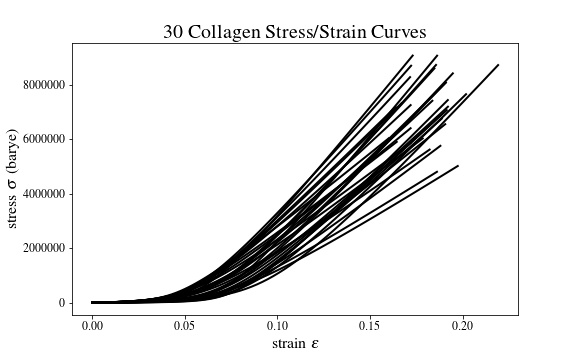
\includegraphics[width=0.45\textwidth]{figures/collagenStressStrain.jpg}
    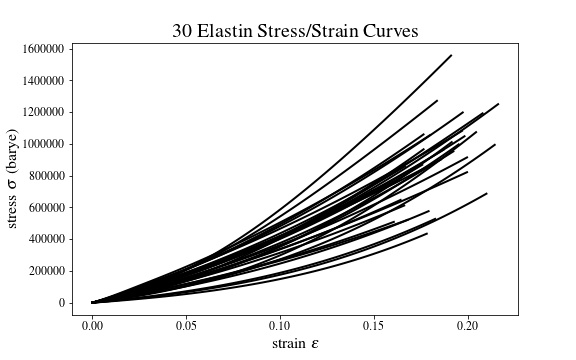
\includegraphics[width=0.45\textwidth]{figures/elastinStressStrain.jpg}
    \caption{Typical stress\slash strain curves for collagen (left) and elastin (right) fibers that make up a septal chord.  Their material parameters have been assigned via statistical distributions.}
    \label{figStressStrainFibers}
\end{figure}

\begin{table}
    \centering
    \begin{tabular}{|l|l|l|l|}
        \hline
        \multicolumn{2}{|c|}{Collagen$\vphantom{|^{|^|}}$} & 
        \multicolumn{2}{|c|}{Elastin} \\ \hline
        $E_1^c$ \hfill [barye] & $5.0 \times 10^{5^{\vphantom{|}}} \pm 2.0 \times 10^5$ &  
        $E_1^e$ \hfill [barye] & $2.3 \times 10^6 \pm 1.0 \times 10^6$ \\
        $E_2^c$ \hfill [barye] & $5.0 \times 10^7 \pm 1.0 \times 10^7$ &  
        $E_2^e$ \hfill [barye] & $1.0 \times 10^7 \pm 2.0 \times 10^6$ \\
        $e^c_t$ & $0.09 \pm 0.015$ &
        $e^e_t$ & $0.4 \pm 0.1$ \\ 
        \hline
    \end{tabular}
    \caption{Physical properties for hydrated collagen and elastin fibers when described with the fiber model of Freed \& Rajagopal \cite{FreedRajagopal16}.}
    \label{tabStressStrainFibers}
\end{table}

Recently, Birzle \textit{et~al}.\ \cite{Birzleetal19} performed experiments on thin slices of rat parenchyma loaded in tension where they removed the collagen and\slash or elastin fiber through collagenase and elastase baths to study their individual behaviors and their interactions under load.
